\chapter{Research}

I propose a framework to examine remixing in an online community of amateur creators. 
I approach this by first studying the design of the online community as a remixing system, and then analyzing what people do and how they react to what others do.
More specifically, I focus on the structural, functional and attitudinal characteristics of an online community's sociotechnical infrastructure and its participants activities.
This framework derives from and is examined through design interventions, three-years of participant observation data, case studies, interviews with community members, quantitative and network analysis of a large corpus of data that includes more than 700,000 registered accounts and a repository of more than 9 million comments and 1.6 million interactive media objects, 30\% of which are remixes.

I study the ways the sociotechnical architecture of a system (Figure~\ref{fig:structure}) influences remixing practices by examining these structural dimensions:
1) granularity of the \ remixable units, 
2) modularity of the remixable components, 
3) decomposability of a finished product, 
4) attributability mechanisms and 
5) openness to remix across systems. 
I analyze these dimensions in the large corpus of data from the Scratch Online Community and by experimenting, for example, with the system's attribution-giving mechanism.

\begin{figure}
\centering
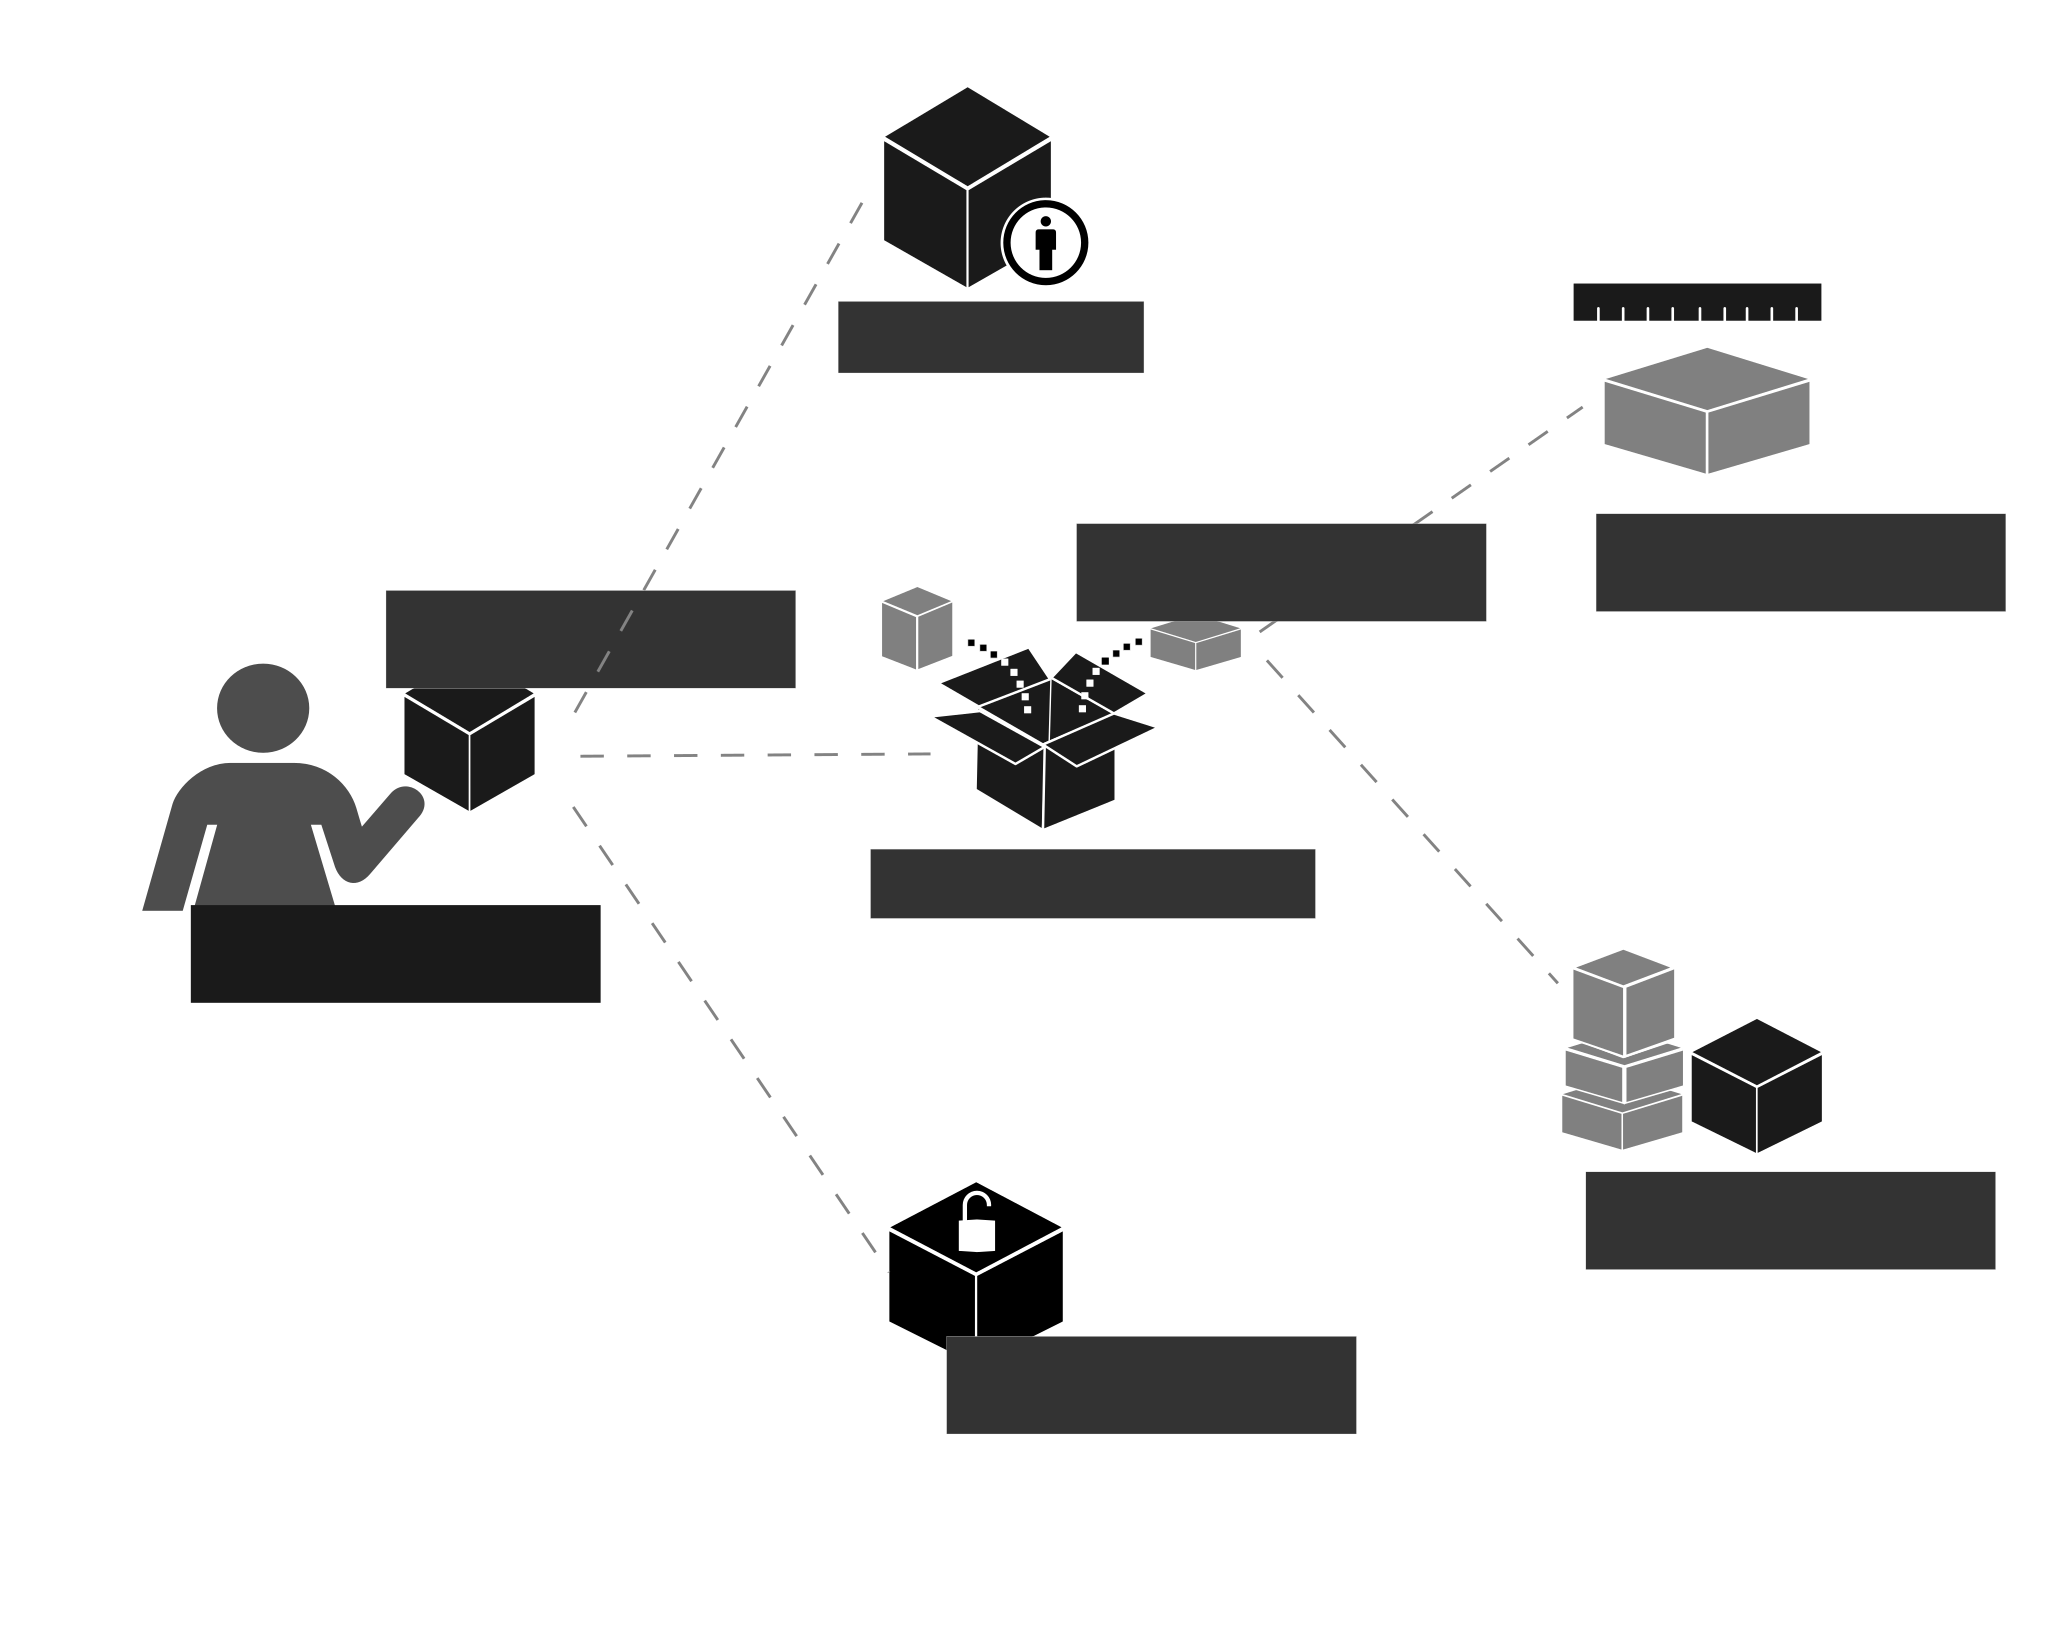
\includegraphics[width=3.25in]{figures/structure.pdf}
\caption{Structural dimensions of a remixing system}
\label{fig:structure}
\end{figure}



I analyze the role remixing plays in participating in an online community of creators.
I look at how several forms of remixing are represented in the Scratch Online Community, how their use evolves, and how they do or do not support sociability and creative practices.
I analyze people's remixing behavior including their: 
1) adding to existing work, 
2) reusing components, 
3) collaborating with others in groups, 
4) persuading crowds to join remixing chains, 
5) inspiring others with ideas for new creations or 
6) self-appropriating their work to create something. 


I investigate remixers' and originators' attitudes toward remixing, in particular, I analyze how participants use or perceive remixing as a cooperative or even 'antisocial' practice and how the system design may influence these attitudes. From the originator's perspective, I look at how and under what circumstances he or she reacts with: 
1) indifference, 
2) acceptance, 
3) encouragement, 
4) conditional acceptance or on an 
5) oppositional attitude. 
Similarly, I look at how remixers may go about remixing: 
1) obliviously, without regard to the norms, 
2) cautiously, or even 
3) antagonistically, as a form of trolling.
I explore these perspectives through case studies and by analyzing people's responses to design interventions intended to support proremixing attitudes and how failures to do so help inform future design repetitions. Analyzing these responses and attitudes can serve as a metric to understand the health of the community and to motivate further design interventions.

% Proposed research:
% How do young people respond to remixing? How are these attitudes represented in the community? When do they embrace remixing and when do they reject it?  I have and will analyze young people’s attitudes based on their own words (interviews) comments, reports (flags) and strategies for deterring (obfuscation, pseudo-licenses, Vigilantism) or supporting remixing (ommenting, scaffolding, framework approach, creation of narratives).
% Crowding out remixing by feaeturing
% Norms: plasticity of virtue
% Evolution of reactions as design changes



